\begin{frame}\frametitle{Введение}
    \heading{YDB -- Open-Source Distributed SQL Database}

    \begin{columns}[onlytextwidth,T]
        \begin{column}{0.5\textwidth}
            \alt<3->
            {
                \textbf<3>{Не только база данных}

                \begin{itemize}
                    \item Платформа, состоящая из различных сервисов
                    \item Таблицы, топики, координация, ...
                \end{itemize}
            }
            {
                \textbf<1>{Распределенная}

                \begin{itemize}
                    \item Обычно запускается на большом кол-ве серверов в разных дата-центрах
                    \item Переживает отказ одного ДЦ + одной стойки в другом ДЦ
                \end{itemize}
            }
        \end{column}

        \pause
        \begin{column}{0.5\textwidth}
            \textbf<2>{Для критичных задач}

            \begin{itemize}
                \item Предназначена для круглосуточной, непрерывной работы
                \item В том числе в периоды обновления и обслуживания
                \item Поддерживает строгую консистентность данных и ACID
            \end{itemize}
        \end{column}
    \end{columns}
\end{frame}

\begin{frame}\frametitle{Введение}
    \heading{Protocol Buffers}

    \begin{columns}[onlytextwidth,T]
        \begin{column}{0.5\textwidth}
            \alt<5->
            {
                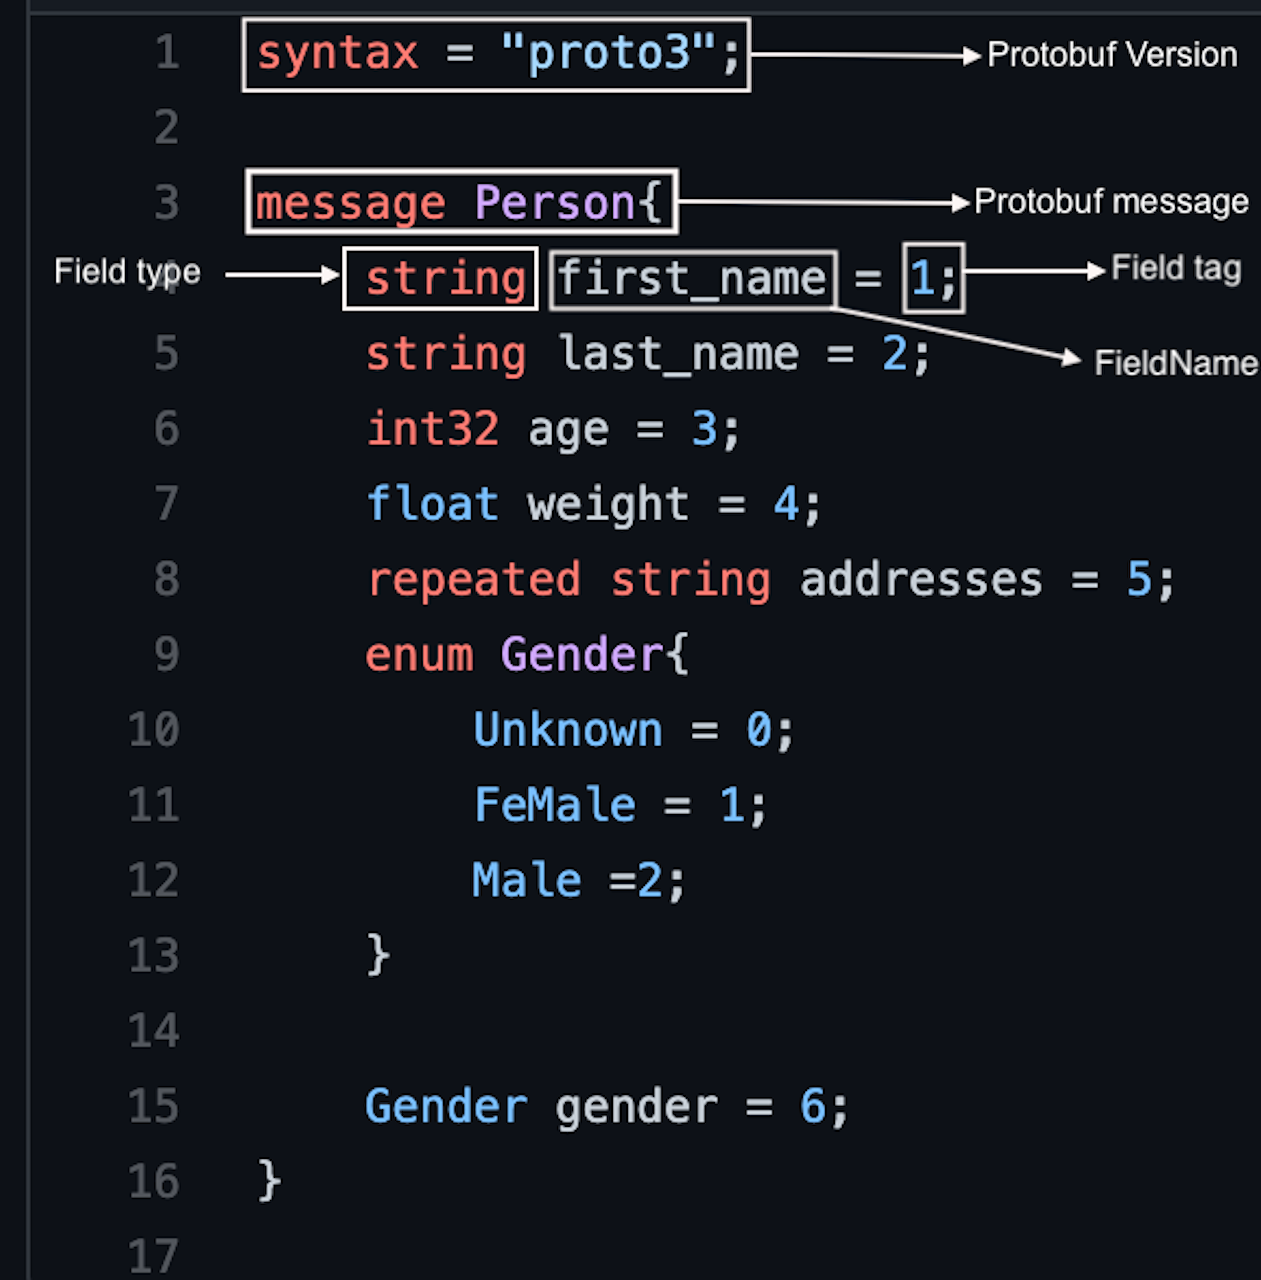
\includegraphics[width=\textwidth]{Protobuf.png}
            }
            {
                \alt<3->
                {
                    \begin{itemize}
                        \item \textbf{IDL (Язык описания интерфейсов)}
                            Позволяет описывать сервисы и сообщения; в результате компиляции получаются определения для
                            выбранного языка программирования:

                            \begin{itemize}
                                \item C++
                                \item Go
                                \item Java
                                \item \alt<4->{Rust}{...}
                            \end{itemize}
                    \end{itemize}
                }
                {
                    \begin{itemize}
                        \item \textbf{Инфраструктура для сериализации}
                            Компилятор собственного IDL + библиотеки для различных платформ и языков программирования
                    \end{itemize}
                }
            }
        \end{column}

        \pause
        \begin{column}{0.5\textwidth}
            \alt<5->
            {
                \begin{itemize}
                    \item \textbf{Модель данных}
                        Сообщения строго типизированные; есть поддержка примитивных и скалярных типов, а также рекурсивных
                        определений.
                \end{itemize}
            }
            {
                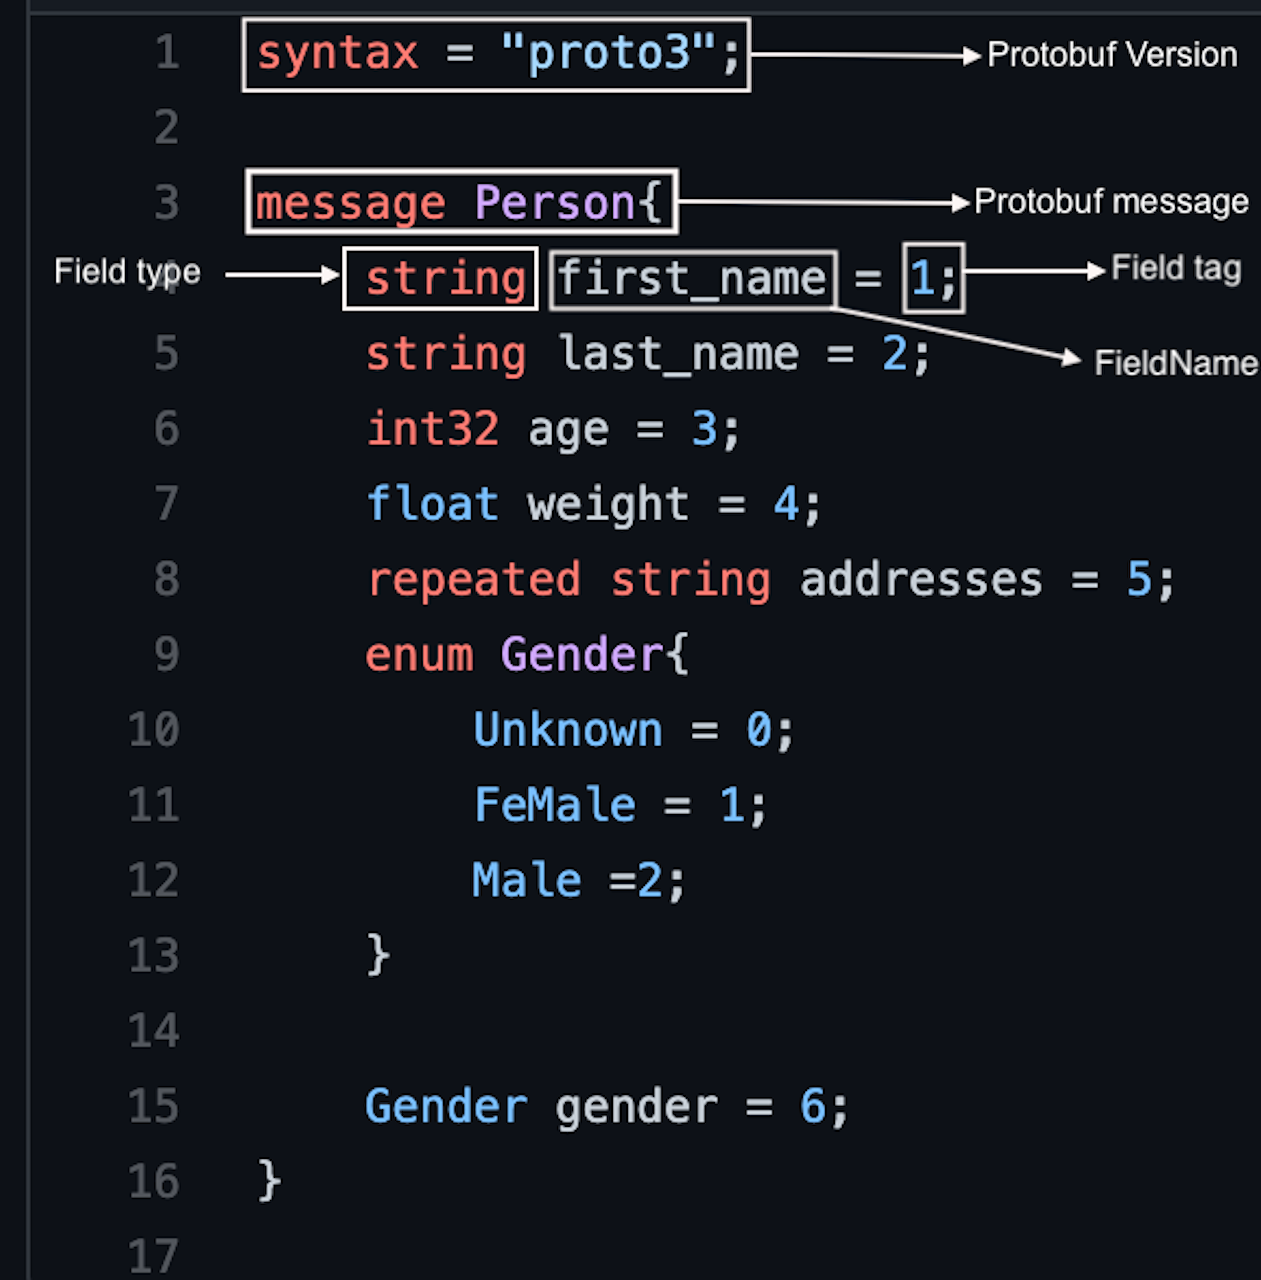
\includegraphics[width=\textwidth]{Protobuf.png}
            }
        \end{column}
    \end{columns}
\end{frame}

\begin{frame}\frametitle{Цель и задачи}
    \begin{block}{В итоге}
        YDB использует Protocol Buffers. За счёт этого для YDB есть SDK на множестве языков программирования.
    \end{block}

    \begin{block}{Цель работы}
        Реализовать поддержку API копирования таблиц в YDB SDK для языка Rust.
    \end{block}

    \begin{block}{Задачи}
        \begin{enumerate}
            \item Реализовать поддержку CopyTables (копирование пачки таблиц)
            \item Реализовать поддержку CopyTable (копирование одиночной таблицы)
        \end{enumerate}
    \end{block}
\end{frame}

\begin{frame}[fragile]\frametitle{CopyTables}
    \begin{lstlisting}
pub async fn copy_tables(
    &self,
    tables: Vec<CopyTableItem>, // { src, dst, omit_indexes }
) -> YdbResult<()> {
    self
        .retry_with_session(RetryOptions::new(), |session| async {
            let mut session = session;
            session
                .copy_tables(tables.to_vec())
                .await?;

            Ok(())
        })
        .await
        .map_err(YdbOrCustomerError::to_ydb_error)
}
    \end{lstlisting}
\end{frame}

\begin{frame}\frametitle{CopyTables}
    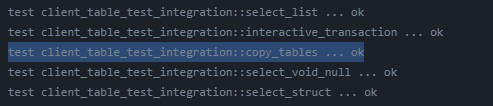
\includegraphics[width=\textwidth]{copy_tables_test.jpg}
\end{frame}

\begin{frame}[fragile]\frametitle{CopyTable}
    \begin{lstlisting}
pub async fn copy_table(
    &self,
    source_path: String, destination_path: String,
) -> YdbResult<()> {
    self
        .retry_with_session(RetryOptions::new(), |session| async {
            let mut session = session;
            session
                .copy_table(
                    source_path.clone(),
                    destination_path.clone(),
                )
                .await?;

            Ok(())
        })
        .await
        .map_err(YdbOrCustomerError::to_ydb_error)
}
    \end{lstlisting}
\end{frame}

\begin{frame}\frametitle{CopyTable}
    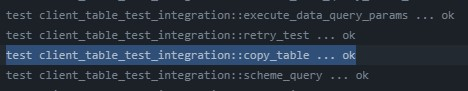
\includegraphics[width=\textwidth]{copy_table_test.jpg}
\end{frame}

\begin{frame}\frametitle{Результаты}
    \begin{itemize}
        \item \textbf{Выполнили все поставленные задачи}
            \begin{itemize}
                \item Реализована поддержка CopyTables (копирование пачки таблиц)
                \item Реализована поддержка CopyTable (копирование одиночной таблицы)
            \end{itemize}
        \item \textbf{Написали unit-тесты для реализованных методов}
            \begin{itemize}
                \item Как было показано ранее, они успешно проходят
            \end{itemize}
    \end{itemize}
\end{frame}
